\chapter{Multi-modal Face Recognition} In biometrics, the classical
definition of ``multi-modal'' refers to the use of more than one
modality or multiple sensors in order to increase the accuracy and
robustness of the biometric recognition system. In this chapter, our
goal is to develop a multi-modal algorithm for face recognition. The
two modalities are the 3-D (shape) and the 2-D (texture) of the
face.

In this dissertation, for the case where the 2-D and 3-D face data
are registered, i.e., correspondences can be established between the
points in 2-D and 3-D data, we develop a multi-modal scheme for face
recognition based on Attributed Relational Graphs (ARG). By using
this technique, the shape and texture are integrated in one graph
model. But in the case where the 2-D and 3-D face data are not
registered, the lack of registration could be due to time laps
between the data acquisition processes such as in case of FRGC data,
we model the 2-D and 3-D face data separately (i.e., ridge images
for shape and ARG model for texture) and then fuse the match results
at the score level. In other words, the process of face recognition
in each modality is accomplished separately, while in the former
scenario, i.e., the 2-D and 3-D data are registered, one model is
built to integrate both the shape and the texture data.

The ARG is a geometric graph with nodes and edges, where the nodes
represent the facial landmarks on the face and the edges connect the
nodes based on the Delaunay triangulation. At each node of the
graph, a set of attributes are extracted from both the shape and the
texture based upon log-Gabor filters. Besides, we define a set of
triangles between the nodes of the graph and a set of features,
i.e., mutual relations, among the sides of the triangles are
defined. The results of face recognition using the 2-D attributes,
3-D attributes, and the mutual relations are fused together in the
score level using various techniques such as the weighted sum rule
and the Dempster-Shafer (DS) theory of evidence.
%
%In the 3-D ARG modeling, we assume that the shape and texture data
%are registered. Therefore, we need to only extract facial landmarks
%from the 2-D images and use them to build the 3-D ARG model. In case
%where the 2-D and 3-D images are not registered, we model the 2-D
%modality of the face using the ARG model, but for the 3-D we use the
%3-D face recognition using ridge images developed in chapter four.
%Then, the results of 2-D and 3-D are fused in the score level to
%enhance the performance of the system.

\section{A Graph Approach For 2-D and 3-D Face Recognition}
Figure \ref{fig_proposed_work} shows the general block diagram of
our system for 2-D and 3-D face recognition based on the ARG model.
We assume that the shape and texture images for each individual
subject in the database are registered. This means that if we
extract the facial landmarks from 2-D images, they match also to the
facial landmarks on 3-D data. The ARG model represents both the 2-D
and the 3-D information within a geometric graph model.

Based on the availability of data from each modality, i.e., 2-D and
3-D, the recognition using only one modality or by fusing data from
the two modalities can be handled easily. In other words, face
recognition problems, such as 2-D versus 3-D, 3-D versus 3-D, and
multi-modal, are approached in a unified manner using the 3-D ARG
model. This multi-modal approach has the potential of minimizing the
problems of pose variations. Specifically, the pose variation
problems can be handled effectively by 3-D information.

\begin{figure}[tbp]
\begin{center}
\epsfig{figure=./chapters/figures/3D_ARG_BDG.eps, width = 6.0 in}
\vskip -1in \caption{General block diagram of our system for face
modeling and recognition based on Attributed Relational Graph.}
\label{fig_proposed_work}
\end{center}
\end{figure}

\section{Graph Modeling} \label{sec_2-D} Elastic Bunch Graph
Matching (EBGM) has shown to be successful in representing complex
objects \cite{Wiskott97, bolme_03}. Wiskott \cite{Wiskott97} modeled
2-D facial images, with pose variations and intensity changes, for
recognition using the EBGM technique. They represent a facial image
by a labeled graph called bunch graph; edges are labeled with
distance information and nodes are labeled with Gabor filter
responses called as jets. In addition, bunch graphs are treated as
combinatorial entities in which, for each fiducial point, a set of
jets from different sample faces are combined, thus creating a
highly adaptable model. This model is matched to new facial images
to reliably find the fiducial points in the image.

There are pros and cons with the EBGM technique. This graph
representation has shown to be successful in face recognition with
good performance rate. But, it is computationally expensive in
extracting the facial features of a new given face image. The edge
representation of the graph in EBGM (i.e., which is simply the
distance between the nodes) is naive and varies under similarity
transformation. In addition, Wiskot \etal \cite{Wiskott97} have
considered all the connections between the nodes to build the graph.
However, there is no need to consider all possible connections
between the nodes (i.e., edges) to build the graph. Since the face
is a geometric object, an optimum set of edges are required to
represent the face using a geometric graph model.

In mathematics, a geometric graph is a graph in which the vertices
or edges are associated with geometric objects or configurations
\cite{Bandelt91, Pisanski00}. A geometric graph, where the vertices
are embedded as points in the Euclidean plane and the edges are
embedded as non-crossing line segments, is called a planar straight
line graph. A triangulation is a planar straight line graph to which
no more edges can be added; a special case of this is the Delaunay
triangulation, a graph defined from a set of points in the plane by
connecting two points with an edge whenever there exists a circle
containing only those two points. Delaunay triangulations maximize
the minimum angle of all the angles of the triangles in the
triangulation. Delaunay triangulation is invariant under similarity
transformation. In addition, perturbing the local position of the
nodes in the graph does not affect the entire configuration of the
graph. This property is useful when representing non-rigid objects
like the face by graph models.

Compared to the EBGM, this technique has some advantages. First, the
edges of the graph are defined based on Delaunay triangulation.
Second, a set of features are extracted and represented using the
edge information. Third, unlike the EBGM, we use an enhanced version
of Active Shape Model technique to find the facial landmarks in the
face, which are used as the nodes of the graph. In the following
sections, we presents in detail our algorithm for face recognition
based on the ARG model.

\subsection{Building the Attributed Graph}
ARG plays an important role in characterizing the content of an
object \cite{park_05}. ARG consists of a set of nodes and mutual
relations between them. Let us denote the ARG by $\mathcal{G} =
(\mathcal{V}, \mathcal{E}, \mathcal{R})$, where $\mathcal{V} =
\{v_1, v_2,\dots,v_N\}$ is the set of nodes of the graph and
$\mathcal{E}=\{e_1, e_2,\dots, e_N\}$ is the set of edges. In this
dissertation, nodes of the graph represent the extracted facial
features on the face and the mutual relations between the nodes are
defined as a set of mutual relations, $\mathcal{R}$, between every
three edges of the Delaunay triangles. The set of mutual relation is
$\mathcal{R}=\{r_{ijk}|e_i,e_j, e_k \in \mathcal{D}_t\}$, where
$\mathcal{D}_t$ is a set of triangles in Delaunay triangulation. In
mathematics, a Delaunay triangulation for a set $P$ of points, is a
triangulation $D_t(P)$ such that no point in $P$ is inside the
circumcircle of any triangle in $D_t(P)$. In other words, we only
consider the mutual relation between three neighboring edges and
these edges are selected based on Delaunay triangulation.

Geometric graphs that are created by Delaunay triangulation are
invariant to scale, in-plane rotation, and translation. In other
words, if an object contains a set of vertices and a set of edges
are defined between the vertices (i.e., edges of the graph) using
Delaunay triangulation, then under the similarity transformation the
set of edges that compose the graph will be the same.

Unlike the work presented by Park \etal \cite{park_05}, where the
nodes of the ARG do not have labels and they rely on stochastic
analysis to find the feature correspondences, the nodes of the ARGs
have direct one-to-one correspondences in our study.
%
%\subsubsection{Texture attributes}  They offer the best simultaneous
%localization of spatial and frequency information.
%
%For texture attributes, at each node of the graph $\mathcal{G}$, we
%calculate the response of the gray scale facial image to a set of
%Gabor filters:
%\begin{eqnarray}\lefteqn{W(x,y,\theta,\lambda,\phi,\sigma,\gamma)=} \nonumber\\
%&exp(-\frac{\acute{x}^2 + \gamma^2\acute{y}^2}{2\sigma^2}).exp[j(\frac{2\pi\acute{x}}{\lambda} + \phi)] \nonumber\\
%&\acute{x}  = x cos\theta + y sin\theta \nonumber \\
%&\acute{y} = - x sin\theta + y cos\theta \label{eq_Gabor}
%\end{eqnarray}where $\theta$ specifies the orientation of the filter, $\lambda$
%is the wavelength of the sine wave, $\sigma$ is the radius of the
%Gaussian, $\phi$ is the phase of the sine wave, and $\gamma$
%specifies the aspect ratio of the Gaussian. The kernel of the Gabor
%filters are selected at eight orientations (i.e.
%$\theta\in\{0,\pi/8,2\pi/8,3\pi/8,4\pi/8,5\pi/8,6\pi/8,7\pi/8\}$)
%and five wavelengths (i.e. $\lambda\in\{1,\sqrt2,2,2\sqrt2,4\}$). In
%order to prevent the filters from having a DC response, we normalize
%the local intensity of the image such that the DC response becomes
%zero. Figure \ref{fig_gabor} shows set of Gabor filter used for
%modeling the texture in this work.
%\begin{figure}[tbp]
%\begin{center}
%\epsfig{figure=./chapters/figures/gabor_wavelet.eps, scale = 0.6}
%\caption{Magnitude response of a set of Gabor filters in five
%wavelengths and eight orientations.} \label{fig_gabor}
%\end{center}
%\end{figure}

\subsubsection{Shape and Texture Attributes}
Gabor filters represent a traditional choice for obtaining localized
frequency information. Gabor filters have similar shapes as the
receptive fields of simple cells found in the visual cortex of
vertebrate animals \cite{Pollen81,Jones87,Devalois88} and can be
statistically derived from images of natural scenes, at least
qualitatively \cite{Olshausen96} \cite{Bell97}.

Gabor filters have two main limitations. The maximum bandwidth of a
Gabor filter is limited to approximately one octave and Gabor
filters are not optimal if one is seeking broad spectral information
with maximal spatial localization. An alternative to the Gabor
function is the Log-Gabor function proposed by Field
\cite{fields87}. Log-Gabor filters can be constructed with arbitrary
bandwidth and the bandwidth can be optimized to produce a filter
with minimal spatial extent. It is worth noting that a Log-Gabor
filter with a three octave bandwidth has the same spatial width as a
one octave Gabor filter, demonstrating the ability of the filters to
capture broad spectral information with a compact spatial filter. In
order to cover the frequency spectrum effectively, a range of both
scales and orientations of the Gabor filters must be considered. The
overall aim is to provide an even coverage of the frequency
components of interest while maintaining a minimum overlap between
filters so as to achieve a measure of independence between the
extracted coefficients \beq \label{eq_log_gabor} \displaystyle G(w)
= e^{-\frac{(log(w/w_0))^2}{2*(log(\sigma/w_0))^2}}\eeq where $w_0$
is the filter's center frequency and $\sigma$ is a scaling factor of
the bandwidth.

To obtain constant shape ratio filters, the term $\sigma/w_0$ must
also be held constant for varying $w_0$. For example, a $\sigma/w_0$
value of .74 will result in a filter bandwidth of approximately one
octave, .55 will result in two octaves, and .41 will produce three
octaves. Figure \ref{fig_logGabor_frequency_resp} shows a set of 1-D
log-Gabor filters seen in logarithmic and linear frequency scales.

\begin{figure}[tbp]
\begin{center}
\includegraphics[scale = .6]{./chapters/figures/logGabor_frequeny.eps}
\caption{A set of 1-D log-Gabor filters seen in logarithmic and
linear frequency scales.}\label{fig_logGabor_frequency_resp}
\end{center}
\end{figure}

There are two important characteristics to note. First, log-Gabor
functions, by definition, always have no DC component, and secondly,
the transfer function of the log Gabor function has an extended tail
at the high frequency end. Field's studies of the statistics of
natural images indicate that natural images have amplitude spectra
that fall off at approximately $1/w$. To encode images having such
spectral characteristics one should use filters having spectra that
are similar. Field suggests that log Gabor functions, having
extended tails, should be able to encode natural images more
efficiently than, say, ordinary Gabor functions, which would
over-represent the low frequency components and under-represent the
high frequency components in any encoding. Another point in support
of the log Gabor function is that it is consistent with measurements
on mammalian visual systems which indicate we have cell responses
that are symmetric on the log frequency scale.

Unfortunately, due to the singularity in the log function at the
origin, one cannot construct an analytic expression for the shape of
the log-Gabor function in the spatial domain. Instead, one designs
the filters in the frequency domain and then perform a numerical
inverse Fourier Transform to see what they look like. Their
appearance is similar to Gabor functions though their shape becomes
much `sharper' as the bandwidth is increased. The shapes of
log-Gabor and Gabor functions are almost identical for bandwidths
less than one octave. Figure \ref{fig_logGabor_spatial} shows two
log-Gabor wavelets of one and two octaves bandwidths all tuned to
the same center frequency.
\begin{figure}[tbp]
\begin{center}
\includegraphics[scale = .6]{./chapters/figures/logGabor_spatial_filters.eps}
\caption{Two pairs of log-Gabor wavelets, odd-symmetric and
even-symmetric (all tuned to the same frequency, $w_0 = 1$, but
having bandwidths of 1 and 3 octaves
respectively.)}\label{fig_logGabor_spatial}
\end{center}
\end{figure}

The 2-D log-Gabor filters are constructed in terms of two
components. The radial component, which controls the frequency band
that the filter responds to and the angular component, which
controls the orientation that the filter responds to. The two
components are multiplied together to construct the overall filter.
The radial component is defined in Equation \ref{eq_log_gabor}.  The
angular component that controls the orientation selectivity of the
filter is simply a Gaussian with respect to the polar angle around
the center frequency. Figure \ref{fig_logGabor_angular} shows a
sample angular component.

\begin{figure}[tbp]
\begin{center}
\includegraphics[scale = .6]{./chapters/figures/logGabor_angular.eps}
\caption{Angular component at angle = 0 and sigma =
1.5.}\label{fig_logGabor_angular}
\end{center}
\end{figure}

Figure \ref{fig_2D_logGabor} shows an example of the even-symmetric
component and odd-symmetric component of 2-D log-Gabor filters in
spatial domain. In our experiments, we use log-Gabor filters with 12
orientations and four scales. The $\sigma/w_0$ is set to .41 which
results in filters with three octaves bandwidth.

\begin{figure}[tbp]
\begin{center}
\includegraphics[scale = .8]{./chapters/figures/2D_log_Gabor.eps}
\caption{Even-symmetric and Odd-Symmetric 2-D log-Gabor filters at
wavelength = 1 with 3 octaves bandwidth.}\label{fig_2D_logGabor}
\end{center}
\end{figure}

\subsubsection{Mutual Relation} For the relation between the nodes,
we define a set of mutual relations (binary/ternary) between every
three nodes that are described by Delaunay triangulation. The first
common type of mutual relations is the angle between the sides of
the triangle. The second type of mutual relations, is the ratio of
the side lengths. These relations are invariant to translations,
rotations, and scale changes \cite{Li92} and are shown to be
powerful for face recognition by Park \etal \cite{park_05}. The
three mutual relations used in this work are defined based on Figure
\ref{fig_Mutual_ARG}:
\begin{eqnarray} &
r_{ijk}(1)=\alpha_1 \nonumber\\& r_{ijk}(2)=min(\alpha_2,\alpha_3) \nonumber\\
& r_{ijk}(3)= (L_1 +  L_2) / (L_1 + L_2 + L_3)
%& r_{ijk}(4)= m_{ijk,x}/\bar{m_x}, r_{ijk}(5)= m_{ijk,y}/\bar{m_y}
\end{eqnarray}

Since the order of the nodes is important in calculating the mutual
relations, a predefined and fixed order of the nodes is used during
the computation of the mutual relations between the nodes.

\begin{figure}[tbp]
\begin{center}
\includegraphics[scale = 0.5]{./chapters/figures/mutual_rel.eps}
\caption{The mutual relation between the
nodes.}\label{fig_Mutual_ARG}
\end{center}
\end{figure}

\subsection{Feature Selection} The number of the features (attributes) play
an important role in the performance of the graph representation for
face modeling and recognition. In this work, we initially extracted
57 landmark points using the improved ASM technique presented in
chapter three. Then, we use a standard template to add more landmark
points at certain positions on the face, such as the cheek and the
points on the ridge of the nose. Extracting these points using the
ASM technique is difficult because of lack of texture in these
regions. The standard template has 109 vertices. By using the
standard template, the total number of landmark points where
representing the nodes of the ARG model is increased to 109. Figure
\ref{fig_landmark_points} shows a sample face in the gallery along
with the points for building the ARG model. We designed an
experiment based on the Sequential Floating Forward Selection (SFFS)
\cite{Pudil94} that searches through the Gabor attributes (there are
109 x 4 x 12 = 5232 attributes for each modality) to find a set of
features which results in the highest performance of the system. The
details of the SFFS algorithm are mentioned in Appendix C.

\begin{figure}[tbp]
\begin{center}
\includegraphics[width = 6.0in, ]{./chapters/figures/109_57_features.eps}
\caption{Extracted landmark points. 57 landmark points (white color)
are extracted by the ASM method and the 52 landmark points (blue
color) are added by aligning a standard template to the facial
points.}\label{fig_landmark_points}
\end{center}
\end{figure}

Figure \ref{fig_SFFS_features} shows the results of feature
selection based on SFFS algorithm. As the results of this analysis,
316 and 999 Gabor attributes are selected for 2-D and 3-D
attributes, respectively. In addition, every node of the graph has
at least one feature which is selected for face recognition.

\begin{figure}
\begin{center}
\includegraphics[width = 5.0 in]{./chapters/figures/feature_selection.eps}
\caption{Results of feature selection for 3-D and 2-D attributes in
the ARG model.}\label{fig_SFFS_features}
\end{center}
\end{figure}

\section{Recognition; Graph Matching} Assume that the ARG models of two faces,
$\mathcal{G}$ and $\acute{\mathcal{G}}$, are given. The similarity
between these two ARGs is defined based on the similarity between
the assigned attributes, i.e., 2-D and 3-D attributes, and the
similarity (dissimilarity) between the mutual relations.

The similarity between two given set of attributes (either 2-D or
3-D) for the graph $\mathcal{G}$ and $\acute{\mathcal{G}}$ are
defined as:

\beq \label{eq_sim_nodes} \displaystyle S_v(\mathcal{V},
\acute{\mathcal{V}}) =
\frac{\sum_{j=1}^{N}a_j\acute{a}_j}{\sqrt{\sum_{j=1}^N a_j^2
\sum_{j=1}^N \acute{a}_j^2}} \eeq where $a_j$ is the magnitude of
the set of complex coefficients of the Gabor attributes, obtained at
the $j^{th}$ node of the graph.

Euclidean distance is used to measure the dissimilarity $D_r(.)$
between the two sets of the mutual relation vectors $\mathcal{R}$
and $\acute{\mathcal{R}}$. Then, the dissimilarity is converted to
similarity by subtracting it from one, i.e., similarity = 1 -
dissimilarity.

\subsection{Pose Normalization}
Prior to building the attributed relational graph, we normalize the
orientation of each deformed 3-D model in the database to be at the
same level of a reference 3-D face model. Figure \ref{fig_pose_3-D}
shows our reference 3-D model with zero degree in pitch, roll, and
yaw angles. We use the extracted facial landmarks by the ASM
technique to estimate the rigid facial pose. Any change in the
pitch, yaw, and roll angles between the captured 3-D model and the
reference model can be accurately computed and used to bring the
deformed model's pose to that of the reference model. Scale
normalization in 3-D is related to how far the object is from the
camera. The further the object is, the smaller it is in the captured
image and vice versa. In order to bring all models at comparable
distances from the capturing camera, hence comparable scales in the
images, we translate the pose normalized 3-D models in depth such
that their depth centroid lie at the mean depth obtained from all
the deformed 3-D models in the database. This insures that all 2-D
facial images are at comparable scales when projected from 3-D.
Figure \ref{fig_pose_normalization_sample} shows the textured 3-D
model of a subject in the UM database before and after
normalization.
\begin{figure}[tbp]
\begin{center}
  \includegraphics[scale = .6]{./chapters/figures/neutral_3D_pose.eps}
  \caption{Neutral 3-D model used to estimate and normalize the pose of a deformed 3-D model.
  The refernce model is at angles (pitch, yaw, roll) = (0,0,0).}\label{fig_pose_3-D}
\end{center}
\end{figure}

\begin{figure}[tbp]
\begin{center}
  \includegraphics[scale = .7, width = 4.0in]{./chapters/figures/normalized_3D_face.eps}
  \caption{3-D textured model (a) before normalization and (b) after normalization.}\label{fig_pose_normalization_sample}
\end{center}
\end{figure}

%Prior to build the attributed relational graph, the raw 2-D facial
%images are processed to normalize the image variations due to the
%effect of lighting and head pose. For lighting normalization, first
%the contrast of image is normalized using histogram equalization.
%Then the intensity value of the image is normalized to have zero
%mean and unit variance. For pose normalization, eye coordinates are
%used to align the faces such that the two eye coordinates of each
%individual facial image is registered to the fixed locations with
%coordinate values (35, 40) and (95, 40) for the right eye and the
%left eye, respectively. This is achieved by applying a 2-D
%transformation i.e., scale, translation and rotation which are
%estimated by procrustes analysis.

\section{Fusing the Information: the 2-D and 3-D Attributes and the Mutual Relation}
In a multi-modal biometric system, fusion is accomplished by
utilizing the information available from different modalities.
Figure \ref{fig_fusion_techniques} shows various types of fusion
that can be used in the context of a biometric system. They can be
categorized as 1) fusion prior to matching and 2) fusion after
matching \cite{Ross06}. The fusion prior to matching integrates
information form multiple sources and can take place either at the
sensor level or at the feature level. In the sensor level fusion,
the raw data from the sensors are combined while in the feature
level fusion, different extracted sets of features from multiple
sources are combined together.

\begin{figure}[tbp]
\begin{center}
  \includegraphics[angle = -90, scale = 0.8]{./chapters/Figures/fusion.eps}
  \caption{Fusion can be accomplished at various levels in a biometric system \cite{Ross06}.}\label{fig_fusion_techniques}
\end{center}
\end{figure}

Schemes for integrating information after the
classification/matching stage can be divided into four categories:
dynamic classifier selection, fusion at the decision level, fusion
at the rank level and fusion at the match score level. A dynamic
classifier selection scheme chooses the classifier which is most
likely to give the correct decision for the specific input pattern.
Integration of information at the abstract or decision level can
take place when each biometric system independently makes a decision
about the identity of the user (in an identification system) or
determines if the claimed identity is true or not (in a verification
system). When each biometric system or modality outputs a match
score indicating the proximity of the input data to a template,
integration can be done at the match score level. This is also known
as fusion at the measurement level or confidence level. Next to the
feature vectors, the matching scores produced by biometric matchers
contain the richest information about the input pattern. Also, it is
relatively easy to access and combine the scores generated by the
different matchers. Consequently, integration of information at the
matching score level is the most common approach in multi-biometric
systems. When the output of each biometric system is a subset of
possible matches (i.e., identities) sorted in decreasing order of
confidence, the fusion can be done at the rank level.

\subsection{Score Level Fusion}
In this work, our aim is to combine the two modalities, 2-D and 3-D
at the score level. We use two different approaches for score
fusion. The first technique is based on the Dempster-Shafer theory
of evidence and the second approach is the weighted sum. Both
approaches are in the category of transform-based techniques (i.e.,
based on the classification presented in \cite{Ross06}.) In
practical multi-biometric systems, an appropriate fusion method is
to directly combine the match scores provided by different matchers
without converting them into posteriori probabilities. However, the
combination of the match scores is meaningful only when the scores
of the individual matchers are comparable. Hence, a transformation
known as score normalization is applied to transform the match
scores obtained from the different matchers into a common domain. In
other words, score normalization refers to changing the locations
and scale parameters of the match score distributions at the outputs
of the individual matchers. Afterwards, the normalized scores of
different matchers can be fused using different rules such as
\textit{Dempster-Shafer theory of evidence}, \textit{weighted sum of
scores}, \textit{maximum scores}, and \textit{minimum scores}.

\subsubsection{Fusion Techniques}
\label{fusion_techniques} One of the well known fusion techniques
used in biometrics is the weighted sum technique which is defined
as: \beq \displaystyle S_f = \sum_{j=1}^{R}w_j*s^n_j
\label{eq_fusion}\eeq where $w_j$ is the weight of the $j^{th}$
modality with the condition $\sum_{j=1}^{R}w_j=1$ and the $s_j$ is
the score of the $j^{th}$ modality. In our case, the weights $w_1$
and $w_2$ and $w_3$ are for the 3-D and 2-D, and mutual relations,
respectively.

The weights can be assigned to each matcher by exhaustive search or
based on their individual performance \cite{Ross06}. The exhaustive
search has shown to be not robust compared to the second approach
where the weights are derived based on individual performance of
each matcher. In this scenario, we assign for each matcher a weight,
which is a function of the matcher's performance derived using a set
of training data. The weights are calculated as follows:

\beq \label{eq_fusion_weights}\displaystyle w_i = \frac{1 - (FAR_i +
FRR_i)}{3 - \sum_{j=1}^{3}(FAR_j + FRR_j)} \eeq where $w_i$ is the
weight for matcher $i$, $FAR_i$, and $FRR_i$ are the false
acceptance rate and the false rejection rate for matcher $i$,
respectively, and $i = 1, 2, and,~ 3$. The values for $FAR_i$, and
$FRR_i$ are threshold dependent. Thus, when the threshold is
changed, the weights assigned to the individual matcher will be
suitably modified.

Another fusion algorithm that is applied to combine the results of
the 2-D and 3-D face recognition is Dempster-Shafer theory
\cite{Shafer76}. A brief overview of DS theory is given below
\cite{premaratne07}.

Let $\Theta = \{\theta_1, \theta_2, ..., \theta_n\}$ be a set of
mutually exclusive and exhaustive propositions that a classifier may
discern. This is referred to as frame of discernment (FoD); it
signifies the ``scope'' of expertise. A proposition $\theta_i$,
referred to as a singleton, represents the lowest level of
discernible information. We use $|\Theta|$ and $2^\Theta$ to denote
the cardinality and the power set of $\Theta$, respectively.
Elements in $2^{\Theta}$ form all the propositions of interest in DS
theory. We use $\bar{A}$ to denote all singletons in $\Theta$ that
are not included in $A$. The ``support'' for proposition $A$ is
provided via a basic belief assignment (BBA) or mass assignment.

The mapping $m : 2^\Theta \longmapsto [0, 1]$ is a BBA for the FoD
$\Theta$ such that: 1) $m(\emptyset) = 0$ and 2) $\sum_{A
\in2^\Theta}m(A) = 1$.

The mass assigned to a proposition is free to move into the
individual singletons that constitute the composite proposition thus
generating the notion of ignorance. The set of propositions
$\mathcal{F}$ that possesses nonzero BBAs forms the focal elements
of $\Theta$; the triple $\{\Theta,\mathcal{F},m\}$ is the
corresponding body of evidence (BoE). The quantity $m(A)$ measures
the support assigned to proposition $A$ only. The belief assigned to
$A$ on the other hand takes into account the supports for all proper
subsets of $A$ as well. Given a BoE, $\{\Theta,\mathcal{F},m\}$, and
$A \subseteq \Theta$, belief is defined as

\beq Bl : 2^\Theta \longmapsto [0, 1] ~~~ where ~ Bl(A) =
\sum_{B\subseteq A}m(B) \eeq

and plausibility is defined as \beq Pl : 2^\Theta \longmapsto [0, 1]
~~~ where ~ Pl(A) = 1 - Bl(\bar{A}). \eeq In other words, in DS
theory, $Bl(A)$ represents the total support that can move into $A$
without any ambiguity; and $Pl(A)$ accounts for all the observations
that do not rule out the proposition $A$. When each focal set
contains only one element, i.e., $m(A) = 0, \forall|A|\neq 1$,
belief functions become probability functions. Then, the BBA, belief
and plausibility all reduce to probability \cite{premaratne04}.

In DS theory, the Dempster's evidence combination function allows
one to combines the evidence generated by several BoEs spanning the
same FoD. Consider BoE1, $\{\Theta_1, \mathcal{F}_1, m_1\}$, and
BoE2, $\{\Theta_2,\mathcal{F}_2,m_2\}$, where $\Theta_1= \Theta_2 =
\Theta$. Then, the Dempster's combination rule generates the BBA
$m(.):2^\Theta \longmapsto [0, 1]  $ for a new BoE as:

\beq \label{eq_ds_rule} m(A) = m(B) \bigoplus m(C) =
\frac{\sum_{B\cap C=A }m(B)_{\Theta_1}m(C)_{\Theta_2}}{1-\sum_{B\cap
C=\emptyset}m(B)_{\Theta_1}m(C)_{\Theta_2}},~~~ \forall A,B,C
\subseteq \Theta. \eeq

This combining rule can be generalized by iteration to fuse more
than two source of information. For example, fusion of three
evidences is defined as: \beq \label{eq_ds_iter} m_{final} = m(B)
\bigoplus m(C) \bigoplus m(D)\eeq where $\bigoplus$ is the DS
combination rule in Eq. \ref{eq_ds_rule}.

In a verification problem (usually in a biometric system, we either
deal with verification or identification), we have two possible
focal elements: ``accept'' and ``reject''. Therefore, the match
score calculated by the face recognition system in the verification
mode after normalization is considered as the mass assignment in DS
theory. Let $s_1$ and $s_2$ be the mass assignment computed from two
face recognition algorithms, then based on the Dempster rule of
combination, the final result is obtained as:

\beq \displaystyle S_{f} = \frac{s_1~s_2}{1 + 2~s_1~s_2~-~s_1~-~s_2}
\eeq Based on Equation \ref{eq_ds_iter}, the above combination rule
can be generalized by iteration to fuse more than two match scores.

Although the above technique works for data fusion, it would be more
realistic when there is a source of uncertainty in making the
decision. For a biometric system in the the verification, usually we
have a certain threshold (i.e., the operating point) and if the
match score is above the that threshold we accept the proposition
otherwise we reject the proposition. However, when the match scores
are close to the operating point threshold (e.g., within $\pm5\%$
from the threshold) then making a decision is uncertain and outcome
might not be accurate. Therefore, for the match scores close to the
operating point of the system, we impose an uncertainty to our
decision. Figure \ref{fig_ds_ambiguity} shows the case where there
is an uncertainty. In this case, we define two thresholds, $T_{low}$
and $T_{high}$ around the operating point. If the match score is
below the $T_{low}$, then we reject that the two given faces under
the test belong to the same identity. If the match score is above
the $T_{hight}$, then when we accept that the two given faces under
the test belong to the same identity. Otherwise, the match score is
in the uncertainty margin and we assign a value to the mass
$m{(``accept'',``reject'')$ based on the lines in Figure
\ref{fig_ds_ambiguity}. The amount of the uncertainty and hence the
new mass assignments in the BoE are calculated as follows.

\beq \label{eq_uncertainty} m(``accept'',``reject'') = a~.~|s
-|~+~b\eeq where $a$ and $b$ are the parameters of the line in
Figure \ref{fig_ds_ambiguity}. After assigning this uncertainty, we
normalize the mass assignment in the BoEs to ensure that the
condition $\sum_{A \in2^\Theta}m(A) = 1$ is achieved.
\begin{figure}[tbp]
\begin{center}
\includegraphics[scale = 1.4]{./chapters/Figures/ds_dual_threshold.eps}
\caption{Dual threshold scenarios and uncertainty in a verification
mode.}\label{fig_ds_ambiguity}
\end{center}
\end{figure}

\section{Experiments and Results}
\label{experiments} In this Section, we present the experimental
results of the methods described above on the University of Miami
face database and the FRGC2.0 database.

\subsection{Experiments on the University of Miami Face Database}
The University of Miami (UM) face database consists of 2-D and dense
3-D facial images of 107 subjects (with neutral expression) were
captured during academic years of 2005-2007 at the University of
Miami. A stereo-based system was designed and developed for 3-D face
modeling (3-D dense reconstruction). At least two sets of images
with the 3-D models exist in the UM database. The first set is used
as the gallery and the second set is used as the probe. For the
details of this database, we refer the reader to the Ph.D.
dissertation of A. Ansari \cite{Nasser07_thesis}.

Figure \ref{fig_UM_database_3-D} shows few subjects in the UM
database including the 2-D images and the 3-D textured model.
\begin{figure}[tbp]
\begin{center}
  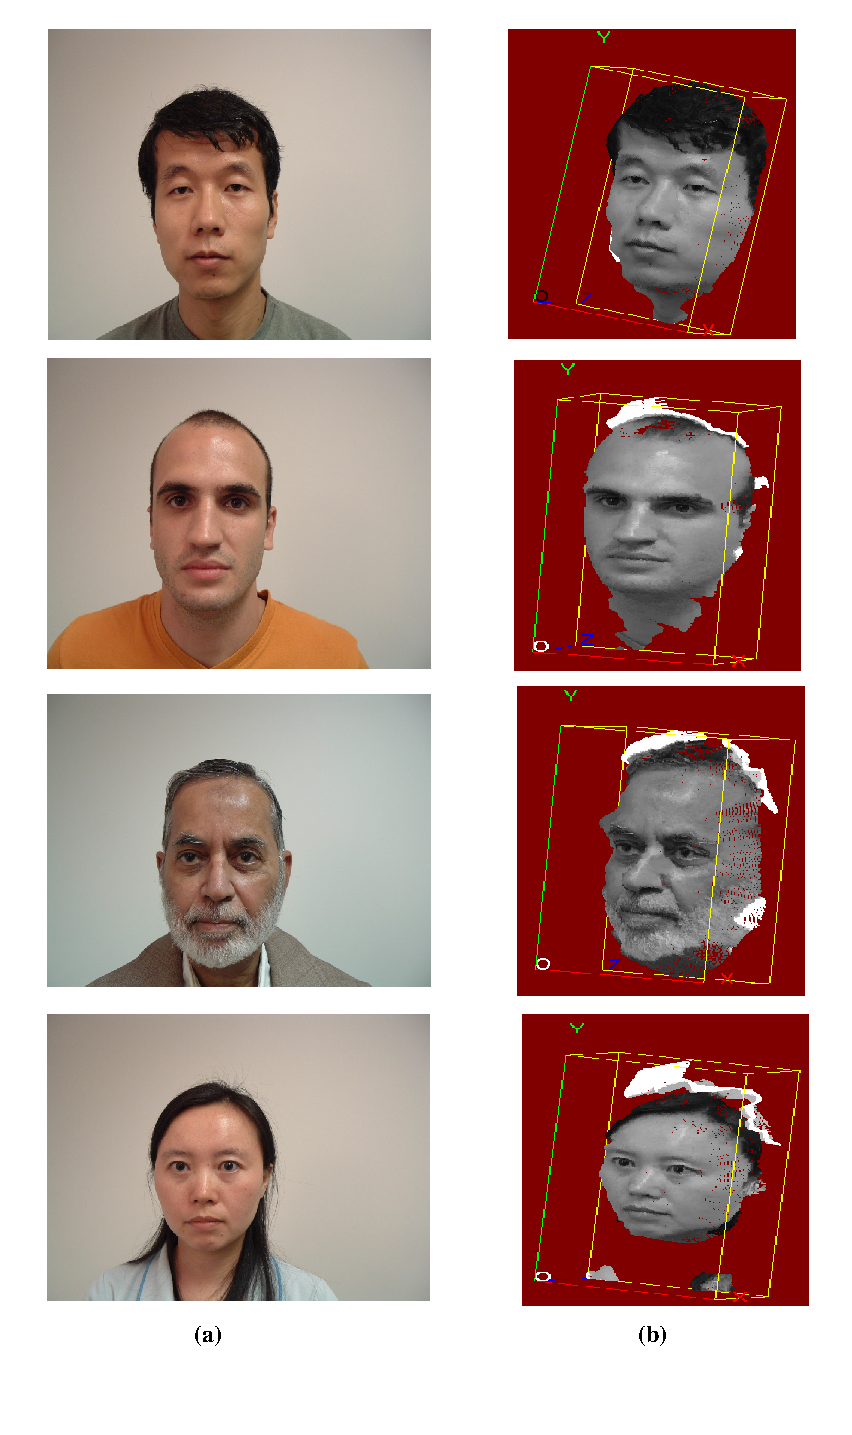
\includegraphics[scale = 0.8]{./chapters/Figures/um_database_samples.eps}
  \caption{Examples of subjects in the UM database: (a) 2-D images and (b) 3-D textured model.}\label{fig_UM_database_3-D}
\end{center}
\end{figure}
\subsubsection{Results}
We tested the performance of our developed system (ARG modeling)
using the UM database. The results of our experiments are reported
in term of the Cumulative Match Characteristic (CMC) curves and the
Receiver Operating Characteristic curves (ROC), for identification
and verification, respectively. Figure \ref{fig_cmc_UM} shows the
CMC curves for the 2-D and 3-D modalities along with the two fusion
techniques (weighted sum and DS theory). The weighting factors in
the weighted sum technique are calculated based on the Equation
\ref{eq_fusion_weights} and are 0.35, 0.34, and 0.31 for the 2-D,
3-D, mutual relations, respectively. The FAR and FRR in Eq.
\ref{eq_fusion_weights} are selected at the Equal Error Rate (EER)
operating point. As the Figure shows, by fusing the mutual relations
with the 2-D and 3-D, the performance of the system is boosted
significantly. In addition, the rank-one identification based on the
DS combination rule and the weighted sum of scores for fusion have
the same performance, 99\%. However, for the verification
experiments, the DS rule of combination outperforms the weighted sum
rule (90\% verification at 0.1\% FAR for the DS rule compared to
81\% verification at 0.1\% FAR for the weighted sum.) Figure
\ref{fig_rank_one_UM} compares the results of rank-one
identification with the work by N. Ansari and M. Abdel-Mottaleb
\cite{Nasser07_thesis}. As shown in Figure \ref{fig_rank_one_UM},
our approach has 99\% rank-one identification rate while the best
performance achieved by Ansari is 96.5\%.)

In addition to the ARG modeling, we applied our developed technique
in chapter 4 (ridge images) to the UM face database. The results of
rank-one identification are presented in Figure
\ref{fig_rank_one_UM}.

\begin{figure}[tbp]
\begin{center}
\includegraphics[scale = .6]{./chapters/figures/cmc_UM.eps}
\caption{Cumulative Match Characteristic curves using the ARG
modeling and two different fusion techniques on the UM
database.}\label{fig_cmc_UM}
\end{center}
\end{figure}

\begin{figure}[tbp]
\begin{center}
  \includegraphics[scale = .6]{./chapters/figures/rank_one_chart_UM.eps}
\caption{Results of rank-one identification using the ARG modeling
and two different fusion techniques on the UM database and the
results of other matching techniques applied to the UM
database.}\label{fig_rank_one_UM}
\end{center}
\end{figure}

Figure \ref{fig_roc_UM} shows the results of verification
experiments on the UM database. The best performance of our system
is achieved by fusion of the different modalities, 91\% at 0.1\%
False Acceptance Rate (FAR).
%%% fig_EER_UM and fig_roc_UM.
\begin{figure}[tbp]
\begin{center}
\includegraphics[scale = .6]{./chapters/figures/roc_UM.eps}
\caption{Receiver Operating Characteristic curves (ROC) using the
ARG modeling and two different fusion techniques on the UM
database.}\label{fig_roc_UM}
\end{center}
\end{figure}

In another experiment, we test the improvement in the performance
our system by adding uncertainty as described by
\ref{eq_uncertainty}. At the operating point of our system (e.g.,
the Equal Error Rate point) we define the uncertainty region as 5\%
above and below this threshold. As a result of adding this
uncertainty and applying the Dempster's combination rule to fuse the
three match scores resulted from ARG modeling, i.e., the 2-D and 3-D
attributes and the mutual relations, the Equal Error rate was
improved 1.8\%. More specifically, the Equal Error rate was 3.5\%
without uncertainty and decreased to 1.7\% by imposing the
uncertainty.

\subsection{Accuracy Analysis of the ARG Model For Face Recognition}
\label{accuracy_ARG} Since, the nodes of the constructed graph in
our work rely on the locations of the feature points and their
correspondences, any error in extraction of the landmark points,
either by the ASM technique, pose estimation, or alignment would
affect the accuracy of the node location/representation and
consequently the performance of the system. We designed an
experiment to analyze the effect of errors in the location of the
nodes on the performance of the system. We add Gaussian noise,
$N(0,\sigma^2)$, to the values of the $x$ and $y$ coordinates of
each node of the graph, which are extracted by the improved ASM
technique. Then we measure the performance of the system for face
recognition based on the noisy constructed ARG models. We only add
noise to the ARG models of the probe images. The results of rank-one
identification are reported for various values of $\sigma$ in Figure
\ref{fig_accuracy_ARG}. As the Figure shows, the 2-D features are
more robust under the effect of noise and the performance of the
face recognition does not drop with even $\sigma = 10$. For the 3-D
features, the performance drops where added noise have a $\sigma$
greater than three. We also learn from this analysis that the mutual
relation features are very sensitive to the noise and the
recognition rate drops rapidly with the increase in $\sigma$.

\begin{figure}[tbp]
\begin{center}
\includegraphics[scale = .6]{./chapters/figures/ARG_noise_analysis.eps}
\caption{Analyzing the robustness of the ARG model in face
recognition with respect to added noise in location of the nodes.
Results of rank-one identification are represented for 2-D, 3-D, and
Mutual relations with respect to various values of $\sigma$ of the
Gaussian noise.}\label{fig_accuracy_ARG}
\end{center}
\end{figure}

\subsection{Experiments on the FRGC V2.0 Face Database}
For a description of the FRGC V2.0 face database, we refer the
reader to Section 4.3.2. Because of the time laps between the 3-D
and 2-D data during the acquisitions for each subjects, the 2-D
(texture) and 3-D (range) images in this database are poorly
registered. Therefore, the extracted locations of the landmark
points in the 2-D images do not correspond to the locations of the
landmark points in 3-D range images. Therefore, instead of modeling
the 3-D (shape) data based on the ARG technique, we use the
developed technique in chapter four for 3-D face matching based on
ridge images. For the 2-D (texture) data, we modeled the face based
on ARG (a 2-D ARG model based on 2-D attributes and mutual
relations.) Then, the results are fused at the score level to obtain
a multi-modal system.

Because the matching scores that results from the 3-D ridge images
are not in the same domain as the other matching scores, they need
to be normalized. After score normalization, the matching scores are
fused based on the technique in Section \ref{fusion_techniques} (the
DS combination rule and the weighted sum rule.)

\subsubsection{Score Normalization}
Two normalization techniques of the matching score that are known to
have high efficiency and robustness are used in this work: the
\textit{Z-Score} and the \textit{Min-Max} normalization functions
\cite{Ross06}. The \textit{z-score} normalization is the most
commonly used normalization technique and is defined as: \beq
\label{eq_z_score} s^n_j = \frac{s_j - \mu_j}{\sigma_j}\eeq where
$s_j$ and $s^n_j$ are the scores before and after normalization,
respectively. $\mu_j$ is the arithmetic mean, and $\sigma_j$ is the
standard deviation for the $j^{th}$ matcher and are estimated using
a training set from the UM database.

The \textit{Min-Max} normalization is defined as: \beq
\large{\label{eq_min_max} s^n_j = \frac{s_j - \min(s_j)}{max(s_j) -
min(s_j)}}\eeq The best performance is achieved by using the
$Min-Max$ normalization technique.

\subsubsection{Results}
Figure \ref{fig_cmc_ARG_FRGC}.a shows the results of identification
in term of CMC curves on the FRGC V2.0 database (the details of the
CMC curves are presented in \ref{fig_cmc_ARG_FRGC}.b.) The results
of 3-D face recognition based on ridges images, the 2-D ARG
modeling, and fusion using the DS combination rule and weighted sum
rule are illustrated in this figure. The results of Rank-one
identification are illustrated in Figure \ref{fig_rank_one_FRGC}.
%
%\begin{figure}[tbp]
%\begin{center}
%  \includegraphics[scale = .6]{./chapters/figures/cmc_FRGC_370.eps}
%  \caption{CMC curves for 2-D, 3-D, Mutual relations features, and
%fusion using DS rule and weighted sum rule for the neutral images
%versus neutral in FRGC V2.0 data-set.}\label{fig_cmc_ARG_FRGC}
%\end{center}
%\end{figure}

\begin{figure}[tbp]
\begin{center}
\begin{tabular}{c}
\epsfig{figure=./chapters/figures/cmc_FRGC_370.eps, scale = 0.45}\label{fig_cmc_frgc_a} \\
(a)\\
\epsfig{figure=./chapters/figures/cmc_FRGC_370_details.eps, scale =
0.5
} \label{fig_cmc_frgc_b}\\
(b)\\
\end{tabular}
\caption{CMC curves (a): for 2-D, 3-D, Mutual relations features,
and fusion using DS rule and weighted sum rule for the neutral
images versus neutral in FRGC V2.0 data-set; (b): the details in
Figure (a).}\label{fig_cmc_ARG_FRGC}
\end{center}
\end{figure}

\begin{figure}[tbp]
\begin{center}
\includegraphics[scale = .6]{./chapters/figures/rank_one_chart_FRGC.eps}
\caption{Results of rank-one identification using the 2-D ARG
modeling, 3-D ridge images, and two different fusion techniques on
the FRGC database.}\label{fig_rank_one_FRGC}
\end{center}
\end{figure}

Figure \ref{fig_results_Neutral_ROC} shows the results of the
verification experiment for the neutral facial images versus the
neutral facial images. The results are presented as Receiver
Operating Curves (ROC) for the two modalities along with the fusion
of the 2-D and 3-D modalities by the weighted sum rule and the DS
combination rule (see Figure \ref{fig_results_Neutral_ROC}). As the
ROC curve shows the 3-D modality has better performance than the 2-D
modality (86.5\% v.s. 74.50\% verification at 0.1\% FAR). In terms
of fusion (3-D + 2-D+Mutual relations), the weighted sum rule has a
comparable performance with the DS combination rule (verification
rate of weighted sum rule and the DS combination rule are 92.5\% and
92.05\% at 0.1\% FAR, respectively.)

\begin{figure}[tbp]
\begin{center}
\includegraphics[scale = 0.6]{./chapters/figures/roc_frgc_370.eps}
\caption{ROC curves for 2-D, 3-D, Mutual relations features, and
fusion using DS rule and weighted sum rule for the neutral images
versus neutral in FRGC V2.0
data-set.}\label{fig_results_Neutral_ROC}
\end{center}
\end{figure}

The result of face recognition using the mutual relations for the
FRGC V2.0 is not significant because the 2-D (texture) images in the
FRGC V2.0 (the dataset in experiment three contains both 2-D and 3-D
data) have poor quality. The main problems with these images are
mainly poor lighting condition, facial hair, closed eyes, and the
occlusion of the facial regions in these images. Figure
\ref{fig_poor_images_frgc} shows few examples of 2-D images with
poor quality in the FRGC V2.0 database. Therefore, locations of the
extracted facial features are not accurate in these poor quality
images. We discussed in Section \ref{accuracy_ARG} that the ARG
model and in particular the mutual relations are sensitive to the
noisy extracted facial features and thus the performance of face
recognition degrades significantly.
\begin{figure}
\begin{center}
\includegraphics[scale = 0.6]{./chapters/figures/poor_images_frgc.eps}
\caption{Samples of facial images in FRGC V2.0 database with poor
quality: (a) closed eyes, (b) facial hair, (c) poor illumination,
(d) occluded facial regions (e) closed eyes and poor illumination
occlusion of facial regions, (f) occluded facial
regions.}\label{fig_poor_images_frgc}
\end{center}
\end{figure}

\section{summary}
We have developed a graph modeling approach called Attributed
Relational Graph (ARG) for modeling the 2-D (texture) and 3-D
(shape) modalities of the face. By using this technique, the shape
and texture are integrated in one graph model. In other words, a
face is modeled by a 3-D geometric graph with nodes and edges such
that the nodes of the graph are the locations of the facial
landmarks on the face. A set of attributes are extracted at the
location of each facial landmark of the face image from both 2-D
(texture) and 3-D (shape) and assigned to the nodes of the graph.
Those attributes are extracted using a set of log-Gabor filters. In
addition to these attributes, a set of geometric features are
extracted based upon the relations between the edge lines in the
graph model. Therefore, each 3-D ARG model of a face contains three
sets of features: 2-D and 3-D attributes at each node and mutual
relations. In order to have a multi-modal system, we have fused the
matching results of the attributes and mutual relations at the score
level. We have utilized the DS theory of evidence and weight sum
rule for fusion. We have tested the performance of the technique
using the University of Miami face database. Our experiments shows
excellent results for face recognition based on the ARG model. For
the case where the 2-D (texture) and 3-D (shape) facial images are
not registered, we modeled the 3-D face data using the ridge images
developed in chapter four. Then, we fused the results of the 2-D
face recognition based on ARG models and 3-D face recognition based
on the ridge images. In addition, our experiments shows that the two
fusion techniques (weighted sum rule and DS combination rule)
utilized in this study have almost the same performance.
